% Full-width teaser under the title. Input by main.tex inside \twocolumn[...] so it lands on page 1.
% Textured renders differ by ~0.8/255 (atlas repacking); bit-identity holds under flat colours only.
\begin{center}
  \centering
  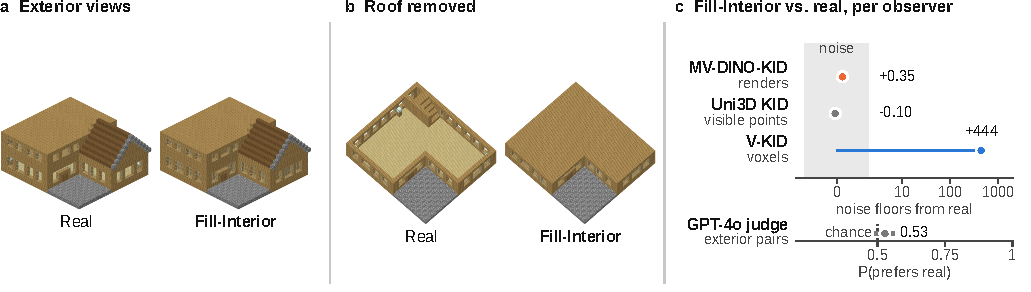
\includegraphics[width=\textwidth]{figures/fig1_teaser}
  \captionsetup{type=figure}
  \caption{\textbf{A metric ranks only what it observes.}
  \textbf{(a)}~A real held-out house and its \solidify{} copy, in which every sealed
  room is filled with the house's own material ($+138\%$ blocks on this build; median
  $+33\%$ over $200$ held-out houses). Rendered in flat colours, the four metric views of this
  build are bit-identical to those of its copy.
  \textbf{(b)}~With the roof removed, the real house has rooms and the copy is solid.
  \textbf{(c)}~Distance of the filled corpus from real data under each observer, in
  noise floors (the shaded band is $\pm 2$). The multi-view DINOv2 KID on exterior
  renders and Uni3D on visible-surface points ($n{=}128$; seeds $-0.1$ and $+0.4$) stay
  inside the noise, and a GPT-4o judge shown exterior pairs prefers the real house in
  $0.53$ of trials ($95\%$ CI $[0.50, 0.56]$). \vkid{} on voxels places the same corpus
  $444$ noise floors away. The render and voxel values come from the $n{=}256$
  leaderboard (\S\ref{sec:complementary}); published builds come from 3D-Craft
  (\suppsec{app:data}).}
  \label{fig:teaser}
\end{center}
